\documentclass[11pt, oneside]{article}   	% use "amsart" instead of "article" for AMSLaTeX format
\usepackage{geometry}                		% See geometry.pdf to learn the layout options. There are lots.
\geometry{letterpaper}                   		% ... or a4paper or a5paper or ... 
%\geometry{landscape}                		% Activate for rotated page geometry
%\usepackage[parfill]{parskip}    		% Activate to begin paragraphs with an empty line rather than an indent
\usepackage{graphicx}				% Use pdf, png, jpg, or eps§ with pdflatex; use eps in DVI mode
								% TeX will automatically convert eps --> pdf in pdflatex		
\usepackage{amssymb}

%SetFonts

%SetFonts
\setlength{\parindent}{0pt}

\title{Summary of Temporal Relational Ranking for Stock Prediction Paper }
\author{Jody Shu}
%\date{}							% Activate to display a given date or no date

\begin{document}
\begin{Large}
\maketitle
%\section{}
%\subsection{}
The authors used a new deep learning solution, named Relational Stock Ranking (RSR) where is able to select the best stock with highest expected revenue.  These are different from other existing deep learning solutions where is to predict stock trend or the stock price and the drawbacks of traditional recurrent neural network (RNN) doesn't look into the relationship between different stocks.  Moreover, the RSR method contributes two key values:
\begin{itemize}
\item Tailoring the deep learning models for stock ranking.
\item Capturing the stock relations in a time-sensitive manner.
\end{itemize}

In this paper, the authors integrate stock relations into prediction, an intuitive solution is to represent the stock relations as a graph and then regularize the prediction of stocks based on the graph (i.e., graph-based learning). However, conventional graph learning techniques cannot capture the temporal evolution property of stock markets (e.g., the strength of influence between two given stocks may vary quickly), since the graph is fixed at a particular time.  Therefore, the authors purpose the ranking task, for which the target is to directly predict a stock list ranked by a desired criteria like return ratio.\\
Please see the figure below from the paper and the descriptions follow. \\
\begin{figure}[h] %  figure placement: here, top, bottom, or page
   \centering
   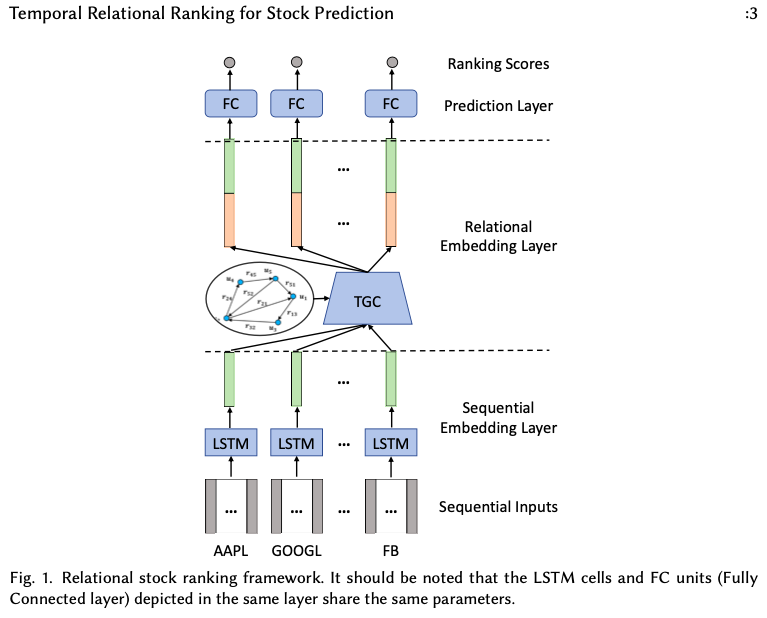
\includegraphics[width=6in]{temporalFig1} 
  % \caption{}
   %\label{fig:example}
\end{figure}

The detail procedure is described by authors as follows:

\begin{itemize}
\item Feed the historical time series data of each stock to a Long Short- Term Memory (LSTM) network to capture the sequential dependencies and learn a stock-wise sequential embedding. 
\item Revise the sequential embeddings by accounting for stock relations in a time-sensitive way (i.e. a new Temporal Graph Convolution (TGC)).
\item Feed the concatenation of sequential embeddings and relational embeddings to a fully connected layer to obtain the ranking score of stocks. 
\end{itemize}



Formally, the LSTM network's transformation module, state vectors, and controlling gates are defined via the following equations:\\

$z_t = \tanh(W_z x^t + Q_z h^{t-1}+b_z)$\\
$i_t = \sigma(W_i x^t+Q_i h^{t-1}+b_i)$\\
$f_t = \sigma(W_f x^t+Q_f h^{t-1}+b_f)$\\
$c_t = f^t \odot c^{t-1} + i^t \odot z^t$\\
$o^t = \sigma(W_o x^t+W_h h^{t-1}+b_o)$\\
$h^t=o^t \odot tanh(c^t)$\\

where $x^t \in \mathbb{R}$ is an input vector, $c^t \ and h^t \in \mathbb{R}^U$ denote the cell state vector and the hidden state vector, respectively, and U is the number of hidden units.  Vector $z^t \in \mathbb{R}^{U}$ is an information transformation module.  Vectors $i^t, o^t \ and \ f^t \in \mathbb{R}^U$ denote the input output and forget gate, respectively. $W_z, W_i, W_f, W_o \in \mathbb{R}$, and $ Q_z, Q_i, Q_f \in \mathbb{R}^{U\times U}$ are mapping matrices; $b_z, b_i, b_f, \ and \ b_o \in \mathbb{R}^U $ are bias vectors.\\


Finally, the key novelty of the authors' work is the proposal of a new component in neural network modeling, named Temporal Graph Convolution, which jointly models the temporal evolution and relation network of stocks.  The experiment was applied on the historical data of two stock markets, NYSE and NASDAQ. Extensive experiments demonstrate the superiority of the RSR method. It outperforms state-of-the-art stock prediction solutions achieving an average return ratio of 98$\% \ and \ 71\%$ on NYSE and NASDAQ, respectively. \\


\end{Large}
\end{document}  